\documentclass[12pt]{article}
\usepackage{geometry}
\geometry{
	left=20mm,
	top=20mm,
}
\usepackage[utf8]{inputenc}
\usepackage{array}
\newcolumntype{C}[1]{>{\centering\let\newline\\\arraybackslash\hspace{0pt}}m{#1}}
\usepackage[spanish]{babel}
 \usepackage{url}
\usepackage[spanish, fixlanguage]{babelbib}
\bibliographystyle{IEEEtran}
\usepackage{graphicx}
\graphicspath{ {./images/} }
\usepackage{amssymb}
\usepackage{amsmath}
\usepackage{subcaption}
\usepackage[linesnumbered]{algorithm2e}
\newcommand\mycommfont[1]{\footnotesize\ttfamily\textcolor{blue}{#1}}
\SetCommentSty{mycommfont}
\usepackage{tikz}
\usetikzlibrary{positioning, fit}
\usetikzlibrary{babel}
\usepackage{titlesec}
\titlespacing*{\section}
{0pt}{5.5ex plus 1ex minus .2ex}{.3ex plus .1ex}
\titlespacing*{\subsection}
{0pt}{5.5ex plus 1ex minus .2ex}{2.3ex plus .1ex}
\title{Tarea 6}

\author{
	Saul Ivan Rivas Vega \\
	\\
	Diseño y análisis de algoritmos\\
\\
	Equipo Completo:\\
		Yadira Fleitas Toranzo\\
		Diego de Jesús Isla Lopez\\
		Saul Ivan Rivas Vega\\
}

\date{\today}

\begin{document}
	\maketitle
	\pagebreak
	\section{Ejercicio 1.}
	  \paragraph{} Sea $T$ un árbol binario con raíz y $S$ un conjunto con un número par de vértices de $T$. Diseña un algoritmo de tipo $divide-y-vencer\acute{a}s$ de tiempo $O(n)$ que empareje los nodos en $S$ de forma tal que en $T$ existan caminos disjuntos en aristas entre cada par.
	  \\ La figura siguiente muestra un ejemplo del problema en el $S$ tiene los seis vértices encerrados en círculos y los emparejamientos se denotan con tres tipos distintos de lineas punteadas.
	  \\
	 \begin{figure}[h]
	 	 \begin{center}
	  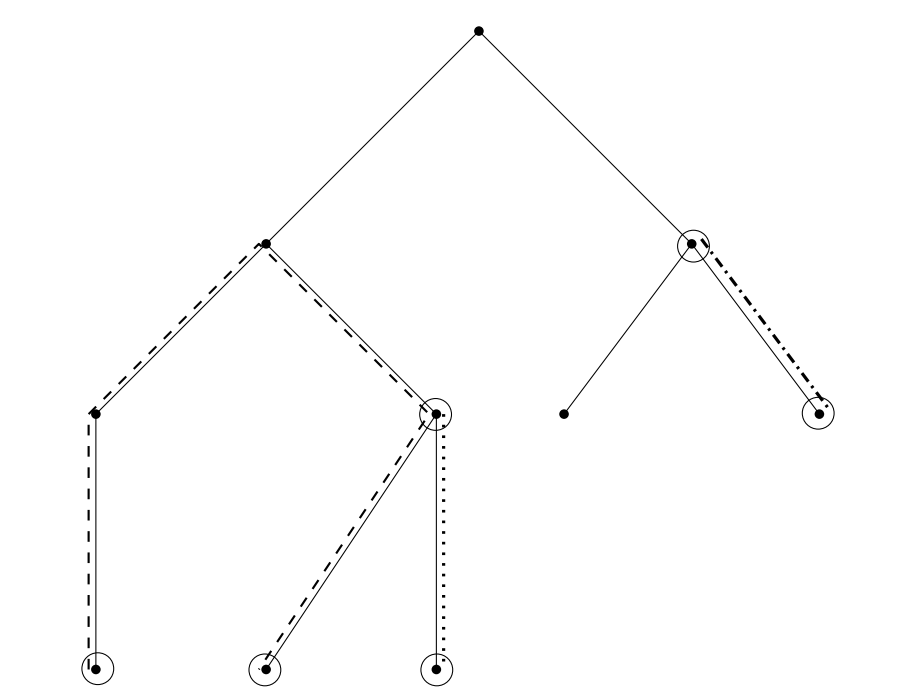
\includegraphics[scale=0.2]{tree_1}
	 	 \end{center}
	  	 \end{figure}
\subsection{Algoritmo}
		\begin{algorithm}[H]\footnotesize
		\KwData{Árbol $T$, donde los nodos tienen adicionalmente un valor True o False si es que pertenecen al conjunto $S$.}
		\KwResult{Conjunto $R$ con las parejas.}
		\SetAlgoLined
		\tcc{Inicializar el conjunto $R$.}
		$R:=\{\}$\;
		\tcc{Llamar la función obtenerParejas' con la raíz del árbol y el conjunto respuesta.}
		obtenerParejas'(raíz, R)\;
		return $R$\;
		\caption{Algoritmo obtenerParejas.}
	\end{algorithm}
\begin{algorithm}[H]\footnotesize
	\KwData{Nodo $u$ y el conjunto actual de parejas $R$.}
	\KwResult{Un nodo que no fue emparejado en el subárbol de $u$, o un valor vacío si no existe dicho nodo.}
	\SetAlgoLined
	\tcc{Inicializar los valores de los nodos sin emparejar encontrados en el subárbol del hijo izquierdo y del hijo derecho, originalmente vacíos} 
	$nodo\_libre\_izq:=\emptyset$\;
	$nodo\_libre\_der:=\emptyset$\;
	\tcc{Realizamos llamadas recursivas en el subárbol del hijo izquierdo y derecho si es que existen} 
	\If{u tiene hijo izquierdo}{$nodo\_libre\_izq$:=obtenerParejas'(hijo izquierdo de $u$, $R$)}
	\If{u tiene hijo derecho}{$nodo\_libre\_der$:=obtenerParejas'(hijo derecho de $u$, $R$)}
	\tcc{Si no hay nodos por emparejar en los subárboles checamos si $u$ tiene que ser emparejado, si es el caso lo devolvemos como nodo por emparejar en su subárbol, en caso contrario devolvemos un valor vacío} 
	\If{$nodo\_libre\_izq$ y $nodo\_libre\_der$ son $\emptyset$}{
		\eIf{u esta en $S$}{
			return $u$\;
		}{return $\emptyset$\;}
	}
	\tcc{En este punto  hay al menos un nodo por emparejar en alguno de los subárboles izquierdo o derecho.} 
 	\tcc{Checamos si $u$ tiene que emparejarse.}
 	\If{u esta en $S$}{
	 	\tcc{Checamos si hubo un nodo libre en el subárbol izquierdo y si es el caso, emparejamos $u$ con ese nodo y devolvemos el valor de $nodo\_libre\_der$ que puede ser vacío o un nodo libre.}
		\eIf{$nodo\_libre\_izq$ no es igual a $\emptyset$}{
			agregamos la pareja $(u, nodo\_libre\_izq)$ a $R$\;
			return $nodo\_libre\_der$\;
		}{
		\tcc{En caso contrario, emparejamos $u$ con el nodo libre en el subárbol derecho y devolvemos un valor vacío.}
			agregamos la pareja $(u, nodo\_libre\_der)$ a $R$\;
			return $\emptyset$\;
		}
 	}
 \tcc{Checamos si existen ambos nodos de los subárboles para emparejarlos o en su defecto retornar el nodo que no este vacío.}
 	\If{no son vacíos $nodo\_libre\_izq$ y $nodo\_libre\_der$} {
 		agregamos la pareja $(nodo\_libre\_izq, nodo\_libre\_der)$ a $R$\;
 		return $\emptyset$
 	}
	return el nodo que no este vacío entre $nodo\_libre\_izq$ y $nodo\_libre\_der$\;
	\caption{Algoritmo obtenerParejas'.}
\end{algorithm}
\pagebreak
\subsection{Demostración complejidad $O(n)$}
El algoritmo 1 realmente no nos dice mucho, solo inicializa el conjunto respuesta y lo retorna al terminar $obtenerParejas'$ el cual es el segundo algoritmo. Por esta razón realizaremos el análisis en el segundo algoritmo.
Cuando el algoritmo es invocado en un nodo hoja, no se realizan mas llamadas recursivas.\\
Esto es, el algoritmo seguirá bajando en en árbol hasta llegar a una hoja, pues antes de realizar una llamada recursiva revisa si tiene un hijo izquierdo o derecho, como se observa en las líneas $3$ y $6$, como una hoja no tiene hijos pues se detendrá ahí.\\
\paragraph{Observación 1} El algoritmo es invocado en un nodo una única vez. Es decir, el algoritmo se llama sobre los hijos del nodo pero en ningún momento se realiza una llamada al padre o a un nodo que no este directamente conectado al nodo actual $u$. Así pues cuando el algoritmo pasa por el nodo $u$, no volveremos a procesar a $u$.\\
\paragraph{Observación 2} Las operaciones realizadas al ser invocado en una hoja, o al regresar de las llamadas recursivas, son de tiempo constante. Es decir que a partir de la línea $9$ hasta el final de las operaciones, solo se realizan comparaciones y asignaciones que podemos considerar de tiempo constante.   \\
Por la observación 1 podemos decir que como existen $n$ nodos, se realizarán $n$ veces las operaciones descritas en la Observación 2 y al ser de tiempo constante decimos que realizamos $n$ veces operaciones de tiempo constante. \\
Finalmente decimos que el algoritmo es de complejidad $O(n)$.
\subsection{Observación} Se pide solo el diseño del algoritmo con la complejidad $O(n)$ en el ejercicio pero se incluye una explicación de porque es correcto.
\paragraph{Correctitud.} 
El algoritmo termina pues por la Observación 1, no se realizarán mas llamadas recursivas al llegar a las hojas, y  en estas solo se toma en cuenta el if en la línea $9$ si es que devolvemos o no al nodo para emparejar. Siendo el número de llamadas $n$ y en cada llamada se realiza un número constante de operaciones.\\
\paragraph{Observación 3} En cada invocación se deja a lo más un nodo sin emparejar  en el subárbol con raíz $u$. Esto lo podemos demostrar por inducción.\\
\textbf{Invariante: } Se deja a lo más un nodo sin emparejar  en el subárbol con raíz $u$ al terminar una invocación.\\
\textbf{Caso base:} Se considera un subárbol de un solo nodo, es decir una hoja. En este caso se devuelve el valor del único nodo si es que tiene que ser emparejado. Se cumple la invariante pues solo podemos devolver el valor del nodo o un valor vacío.\\
\textbf{Hipótesis inductiva:} En cada invocación intermedia podemos emparejar los nodos libres que existan en el subárbol, de tal forma que dejemos a lo más uno libre.\\
Suponer verdadero hasta algún nodo intermedio en el árbol $T$.\\
Dicha invocación en el nodo $u$ tiene los siguientes casos:
\begin{enumerate}
	\item \textbf{u no tiene que emparejarse}
	\begin{enumerate}
		\item La invocación del hijo izquierdo si devolvió un valor no vacío y también la invocación en el hijo derecho. En este caso se emparejan dichos nodos y no quedan nodos libres.
		\item Alguna de las dos invocaciones en los hijos devolvió un valor no vacío y otro sí. En este caso queda libre el nodo que no fue vacío de las invocaciones.
		\item Ninguna de las dos invocaciones en los hijos devolvió un valor no vacío. En este caso no quedan nodos libres.
	\end{enumerate}
	\item \textbf{u si tiene que emparejarse}
	\begin{enumerate}
		\item La invocación del hijo izquierdo si devolvió un valor no vacío y también la invocación en el hijo derecho. En este caso se emparejan el nodo $u$ con el nodo libre de la invocación en el hijo izquierdo, dejando libre el nodo de la invocación en el hijo derecho.
		\item Alguna de las dos invocaciones en los hijos devolvió un valor no vacío y otro sí. En este caso se empareja la el nodo $u$ con el nodo libre de las invocaciones y no quedan nodos libres.
		\item Ninguna de las dos invocaciones en los hijos devolvió un valor no vacío. En este caso queda libre el nodo $u$.
	\end{enumerate}
\end{enumerate}
Finalmente como en ninguno de los casos se termina con dos o mas nodos libres podemos decir que en cada invocación se deja a lo más un nodo sin emparejar  en el subárbol con raíz $u$.\\
Probemos ahora que las parejas resultantes no comparten aristas en el camino que las conecta.\\
Por contradicción.\\
Entonces significa que hay por lo menos una arista por el cual pasan 2 caminos entre parejas. \\
Tomemos el subárbol $T_j$ el cuál tiene como raíz al nodo inferior en dicha arista. Tal como se muestra en la figura siguiente.\\
\begin{figure}[h]
\begin{center}
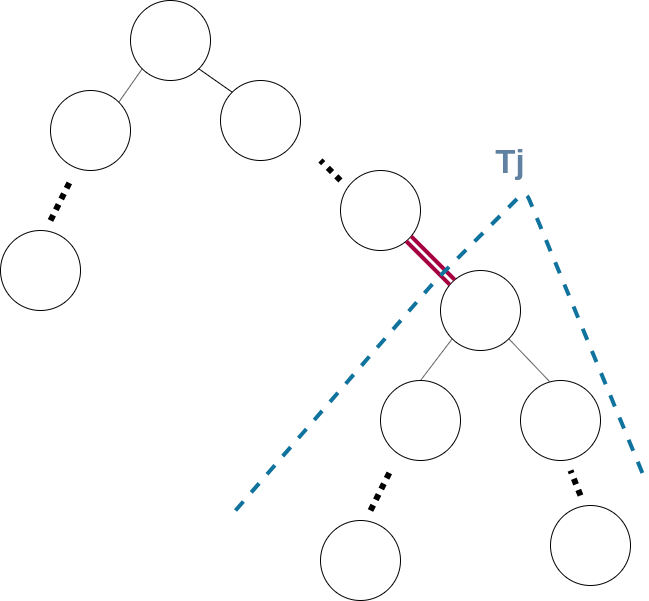
\includegraphics[scale=0.5]{ARBOL}
	\end{center}
\caption{Subárbol $T_j$ (línea punteada), arista con doble camino (en rojo).}
\end{figure}
\pagebreak
\paragraph{} Eso quiere decir que en el subárbol $T_j$ existen por lo menos 2 nodos cuyas respectivas parejas se encuentran fuera de $T_j$. Si tomamos la invocación del algoritmo en la raíz de $T_j$, para que cumpla que las parejas de esos 2 nodos no están en $T_j$, al terminar dicha invocación debió dejar esos 2 nodos libres. Sin embargo esto es una contradicción ya que por la Observación 3 al terminar una invocación se deja a lo mas 1 nodo libre en el subárbol.\\
Finalmente como no puede existir ni una sola arista por el cual pasan dos caminos entre parejas decimos que  las parejas resultantes no comparten aristas en el camino que las conecta.\\
\section{Ejercicio 2.}
\section{Ejercicio 3.}
Se tienen dos bases de datos, $BD_1$ y $BD_2$, cada una con $n$ valores numéricos distintos, en total $2n$ valores distintos. La única manera de accesar los datos es mediante preguntas, en las cuales se le da un valor $i\in\{1,..., n\}$ a una de las dos bases de datos, $BD_j$, y esta responde con el $i$-ésimo valor más pequeño que contiene $BD_j$. Diseña un algoritmo que dado un entero $k\in\{1,...,2n\}$ de entrada, encuentre el $k$-ésimo valor más pequeño en las bases de datos, usando $O(logn)$ preguntas. Demuestra la correctez y complejidad de tu algoritmo.
\subsection{Algoritmo}
\begin{algorithm}[H]\footnotesize
	\KwData{Número $k$.}
	\KwResult{El $k$-ésimo elemento de entre las dos bases de datos.}
	\SetAlgoLined
	\tcc{Inicializar los índices inicio y final para la busqueda binaria.}
	$inicio:=0$\;
	$fin:=k$\;
	\tcc{Mientras el inicio sea menor o igual al final.}
	 \While{inicio $\leq$ fin}{
		 \tcc{Obtenemos el valor en la mitad en el rango de los índices.}
		 mitad:=(inicio + fin) / 2\;
		 \tcc{El valor 'mitad' funciona para representar cual valor se encuentra en esa posición en la primera base de datos y los restantes en la segunda base de datos. Es decir el $k$-ésimo elemento es aquel que es mayor a (mitad + (k-mitad)) - 1, elementos.}
		 tomados\_bd1:=min(n, mitad)\;
 		 valor\_bd1:=PREGUNTAR\_BD1(tomados\_bd1)\;
 		 tomados\_bd2:=min(n, k -tomados\_bd1)\;
  		 valor\_bd2:=PREGUNTAR\_BD2(tomados\_bd2)\;
  		 \tcc{Ahora si la cantidad de elementos es igual  a $k$ (es decir que es mayor a la cantidad necesaria de elementos).}
  		\eIf{tomados\_bd1 + tomados\_bd2 es igual a $k$}{
  			\tcc{Veamos si es que el elemento que le sigue en la base de datos 2 es menor al valor de la izquierdo, lo que causaría que sea mayor que mas de $k$ elementos.}
  			valor\_check\_bd2:=PREGUNTAR\_BD1(tomados\_bd2 + 1)\;
  			\eIf{valor\_check\_bd2 $>$  valor\_bd1}{
  				\tcc{Si en efecto no fue menor entonces ya tenemos $k$ elementos donde el mas grande es el mayor de entre el valor que obtuvimos de las bases de datos.}
  				return max(valor\_bd1, valor\_bd2)\;
  			}{
  				\tcc{En este caso tendremos mas de $k$ elementos. Por lo tanto debemos buscar un índice más pequeño}
  				fin:= mitad-1\;
  			}
  		}{
  			\tcc{En este caso tendremos menos de $k$ elementos. Por lo tanto debemos buscar un índice más grande}
  			inicio:= mitad+1\;
  		}
	 }
	\caption{Algoritmo $k$-ésimo elemento.}
\end{algorithm}
\subsection{}\paragraph{Correctitud.} 
El algoritmo termina pues en los condicionales de las líneas $9$ y $11$ si se cumplen ambas se devuelve el valor encontrado, siendo este el mayor de entre los consultados en la base de datos 1 y 2. Y en caso de que al menos una no se cumpla el espacio de búsqueda es reducido por la mitad, terminando en $logn$ pasos.\\
El algoritmo devolverá el $k$-ésimo valor más pequeño en las bases de datos.\\
Por inducción.\\
\textbf{Invariante: } El $k$-ésimo elemento es mayor a $x$ elementos en la base de datos 1 y a $(k-x-1)$ elementos en la base de datos 2, tal que $inicio \leq x \leq fin$ .\\
\textbf{Caso base:} Se considera la primera pregunta en el algoritmo, el rango es $inicio=0$ y $fin=k$, y naturalmente el valor $x$ que buscamos se encuentra en dicho rango pues la menor cantidad de elementos al que puede ser mayor es 0 y la máxima los $k$ elementos, es decir los $2n$ elementos.\\
\textbf{Hipótesis inductiva:} Si el valor $x$ que búscamos no es igual al valor 'mitad' actual, se encuentra ya sea en el rango $(inicio, mitad - 1)$ o en el rango $(mitad + 1, fin)$.
Suponer verdadero hasta la $i$-ésima pregunta.\\
Tomemos al valor 'mitad' y tomemos el valor de preguntárselo a la primera base de datos. Cualquier valor en la base de datos 1 con un índice mayor a 'mitad' es mayor al valor que esta en 'mitad', por definición. Veamos el valor en exactamente la cantidad de elementos restantes, es decir a $(k-mitad)$ en la base de datos 2. Ahora cualquier valor en la base de datos 2 con un índice mayor a $(k-mitad)$ es mayor al valor que esta en $(k-mitad)$, por definición. Sin embargo no necesariamente son mayores al valor en $mitad$ en la base de datos 1. \\
Si tomamos el caso donde si es mayor entonces el mayor de los revisados en las bases de datos es la respuesta, puesto que si tenemos k elementos entre $mitad$ y $k-mitad$, y ademas no hay elementos menores a los comprendidos en ellos, el k-ésimo elemento es el mayor de ambos.\\
En caso contrario el valor significa que si tomamos a $mitad$ en la base de datos 1 tendremos por lo menos $mitad +k-mitad + 1$ elementos, lo cual es mayor a $k$, por lo tanto si reducimos el valor que estamos considerando como $mitad$ reduciremos la cantidad de elementos a los que es mayor. Como se observa en la línea $14$.\\
Análogamente si terminamos con menos elementos si aumentamos $mitad$ aumentaremos la cantidad de elementos a los que es mayor. Como se observa en la línea $17$.\\
Entonces como el rango se adapta dependiendo si se tienen mas o menos elementos de los necesarios, decimos que $x$ se encuentra en $(inicio,fin)$.\\
Finalmente como el rango se reducirá, de no encontrarlo todavía llegará al punto donde el rango comprende solo a un elemento siendo este el valor $x$ buscado.\\
\paragraph{Complejidad en tiempo (cantidad de preguntas).} Se realizan 3 preguntas en cada iteración del while, y el while reduce por la mitad el rango de búsqueda. El rango originalmente es de tamaño $k$, por lo tanto se realizan $logk$ iteraciones. Le sigue que son $3logk$ preguntas, y como $k=2n$, es como si tuviéramos $3(log2 + logn)$. Es decir $3(1 + logn)=3 + logn$.  Esta cantidad de preguntas es de orden $O(logn)$. Sin embargo para un análisis temporal completo tendríamos que multiplicar esa cantidad de preguntas por la función de complejidad de cada pregunta. 
\section{Ejercicio 4.}
En clase revisamos el algoritmo de los códigos de Huffman. En el primer intento de prueba, quisieron probar que el árbol $T$ que generaba el código encontrado satisfacía:
\begin{enumerate}
	\item  $T$ es completo.
	\item Si $a$ y $b$ son hojas del árbol tales que profu$(a)$ $<$ profu$(b)$ entonces $f_a \geq f_b$ ($f_x$ es la frecuencia con que aparece $x$ en el texto).
	\item Los dos símbolos de frecuencia menor son hermanos en $T$.
\end{enumerate}
Demuestra que esa estrategia no funciona para probar lo que queríamos. Es decir, ofrece un alfabeto $S$ con frecuencias $f:S\rightarrow[0,1]$ y encuentra un código $\varphi$ que no sea óptimo y cuyo árbol generado satisfaga las tres propiedades anteriores. Demuestra por qué el código que propones no es óptimo.\\
Nota: La prueba vista en clase de hecho muestra que la propiedad arriba mencionada se cumple no solo para el árbol $T$ con $n$ hojas, sino para el árbol $T'$ que junta $a$ y $b$ en un solo símbolo. 
\subsection{}
\begin{figure}[h]
	\begin{center}
		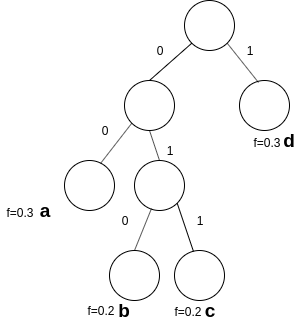
\includegraphics[scale=0.5]{codificacion}
	\end{center}
	\caption{Codificación no óptima que cumple con las propiedades.}
\end{figure}
Ahora con esta codificación obtengamos las sumas de la longitud por la frecuencia:
\begin{equation}
Suma_a = 0.3 \times longitud(00) = 0.3 \times 2 = 0.6
\end{equation}
\begin{equation}
Suma_b = 0.2 \times longitud(010) = 0.2 \times 3 = 0.6
\end{equation}
\begin{equation}
Suma_c = 0.2 \times longitud(011) = 0.2 \times 3 = 0.6
\end{equation}
\begin{equation}
Suma_d = 0.3 \times longitud(1) = 0.3 \times 1 = 0.3
\end{equation}
Si sumamos todo para obtener $AVG(T)$ tenemos:
\begin{equation}
AVG(T)= 0.6 + 0.6 + 0.6  + 0.3 = 2.1
\end{equation}
\subsection{}
Ahora tomemos una codificación óptima:
\begin{figure}[h]
	\begin{center}
		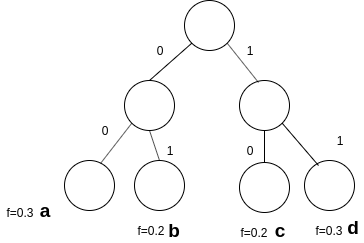
\includegraphics[scale=0.5]{codificacion2}
	\end{center}
	\caption{Codificación óptima que cumple con las propiedades.}
\end{figure}
Ahora con esta codificación obtengamos las sumas de la longitud por la frecuencia:
\begin{equation}
Suma_a = 0.3 \times longitud(00) = 0.3 \times 2 = 0.6
\end{equation}
\begin{equation}
Suma_b = 0.2 \times longitud(01) = 0.2 \times 2 = 0.4
\end{equation}
\begin{equation}
Suma_c = 0.2 \times longitud(10) = 0.2 \times 2 = 0.4
\end{equation}
\begin{equation}
Suma_d = 0.3 \times longitud(11) = 0.3 \times 2 = 0.6
\end{equation}
Si sumamos todo para obtener $AVG(T)$ tenemos:
\begin{equation}
AVG(T)= 0.6 + 0.4 + 0.4  + 0.6 = 2.0
\end{equation}
Finalmente como en efecto existe una codificación con menor $AVG$ que la primera codificación entonces no es óptima aún cuando cumple con las 3 propiedades.
\end{document}  